% !TEX encoding = UTF-8 Unicode
% !TEX root = rapport.tex

\chapter{Initiatives et solutions}\label{initiatives_actuelles}

\section{Initiatives des pouvoirs publics}

\subsection{Mesures des pouvoirs publics français}
\subsubsection{Le C2i}

Mis en place à partir de la rentrée universitaire 2003
\cite{circulaire_c2i}, le certificat informatique et internet (C2i)
vise à encadrer la formation des étudiants aux technologies
informatisées et à internet par l'établissement d'un socle commun.

\begin{figure}[H]
  \centering
  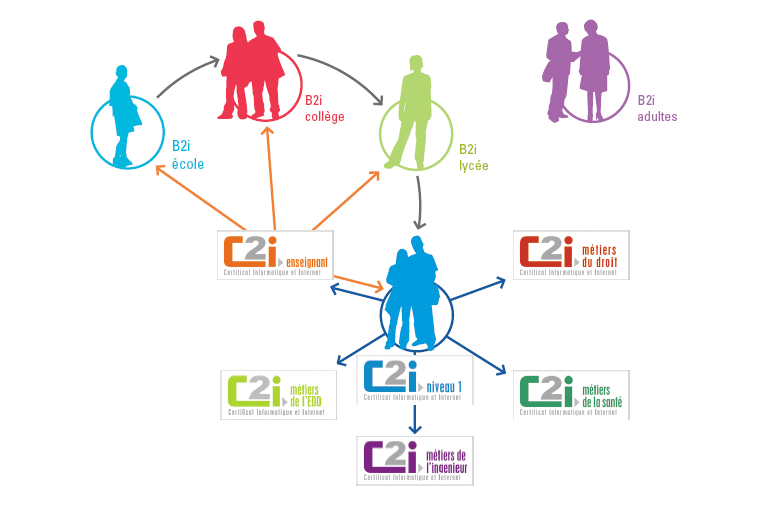
\includegraphics[width=\textwidth]{../resources/illustrations/c2i}
  \caption{Différents niveaux et spécialités du C2i}
\end{figure}

\cite{b2i_c2i}
\cite{b2i}
\cite{isn}

\subsubsection{Les opérations "ordinateurs portables"}

Les opérations \og{}ordinateurs portables\fg{} sont à la mode au
lycée. OrdiLib' en Midi-Pyrénées, Ordipass en Pays de la Loire, LoRdi
en Languedoc-Roussilon, ces initiatives des régions visent à fournir à
chaque lycéen l'accès à un ordinateur portable personnel.

\cite{portables35}
\cite{portables60}
\cite{portables40}


\subsubsection{Le rapport \og{}Refondons l'école de la république\fg{}}

Nous avons vu différentes actions mené par le gouvernement ou les
régions afin d'une part de former les étudiants au NTIC et d'autres
part de favoriser l'utilisation des NTIC dans le système éducatif. Nous
allons maintenant nous intéresser aux propositions pour l'avenir de
l'éducation à travers la concertation \og{}Refondons l'école de la
république\fg{} confié par le gouvernement Ayrault à Nathalie Mons, Christian
Forestier, François Bonneau et Marie-Françoise Colombani. Il ressort à
travers se rapport plusieurs thèmes tels que \og{}apprendre à
apprendre\fg{}, \og{}une appropriation active des langues\fg{},
\og{}usages pédagogiques du numérique en primaire\fg{}, \og{}une
évaluation positive, plutôt qu'une note sanction\fg{}… Ces différents
thèmes sont des points d'interrogation cruciaux pour l'école de demain,
nous regretterons cependant un manque de mesures concrètes. Nous
pouvons tout de même relevé la volonté d'inscrire dans la loi \og
l'éducation au médias et à l'information\fg{}, de mettre en place un plan
pour l'éducation numérique au primaire, de former les enseignants aux
usages pédagogiques du numérique, de mettre en place une politique
publique de recherche dans le cadre des applications pédagogiques du
numérique.


\subsection{Mesures des pouvoirs publics internationaux}
Forum mondial sur l’éducation \cite{educ_forum}
Les TIC au service de l’éducation \cite{tics}
Un regard sur la trajectoire de l’informatique éducative au Brésil \cite{peixoto2006regard}
Willem J. PELGRUM, Arian T. SCHIPPER, "Indicators of computer integration in education" \cite{pelgrum1993indicators}


\section{Initiatives d'autres acteurs}

D'autres actions, souvent plus radicales ont lieu à travers le monde. Elles sont menées en général par des chercheurs dans les domaines de l'informatique. Elles amènent à une réelle remise en question du système éducatif et plus généralement des réflexions poussées sur les méthodes d'apprentissage.

\subsection{Des expérimentations basées sur le constructivisme}
\textit{Présentation du constructivisme}

\subsection{Actions concrètes}
\textit{Présentation de quelques actions menées à travers le monde}
\subsubsection{Pays en développement}
\subsubsection{Accès à la technologie}
\textit{OLPC}
One Laptop Per Child (OLPC) est une association à but non lucratif
présidée par Nicholas Negroponte ancien professeur au MIT où il a
notamment crée le MediaLab. En 2005, il annonce le lancement d'un
projet de recherche consistant au développement d'un ordinateur
portable d'une valeur de 100\$ dans le but de les distribués ensuite
dans les pays défavorisés.

\subsubsection{e-learning / e-teaching}
\textit{Moodle -- AI-class}
Les plate-formes d'apprentissage en ligne \og{}e-learning\fg{} tels
que Moodle, udacity, kanacademy, coursera, MIT Open Courseware, etc.,
émergent depuis ces dernières années. Ce type d'apprentissage offre l'avantage d'être peu
coûteux, flexible dans la gestion du temps d'apprentissage, largement
accessible. Loin de remplacer l'enseignement traditionnel, ce type
d'apprentissage offre un complément voir un support à celui-ci. Ce
type de support est souvent utilisé pour de la formation continue
qu'elle soit professionnel ou personnelle.

\subsubsection{Auto-apprentissage}
\textit{Hole in the wall}

\section{Quelles peuvent être les solutions adaptées pour endiguer le phénomène ?}\label{solutions}

Interactions entre professeur et élèves
Révision des programmes
Utilisation des nouvelles technologies au service des interactions
Changements des règles de constitution des classes : pourquoi par tranches d'âge ?
Personnalisation des parcours en fonction des envies des élèves.

\subsection{Classification des élèves par besoins / capacités  et non par tranche d'âge}
\subsection{Amélioration de la pertinence des évaluations}
\subsection{Prise en compte des besoins de coopération sans parler de triche}

